\documentclass{article}
\usepackage[UTF8]{ctex}
\usepackage{amsmath,mathtools,geometry,pgfplots,float,mathrsfs,caption,enumerate}
\pgfplotsset{compat=1.15}
\usetikzlibrary{arrows}
\geometry{scale=0.7}

\newcommand\cusong[1]{
	\noindent \rlap{\hspace{0.01em}#1}\rlap{\hspace{0.02em}#1}\rlap{\hspace{0.03em}#1}\rlap{\hspace{0.04em}#1}\rlap{\hspace{0.05em}#1}#1
}

\title{\vspace*{-1em}\cusong{每日一题(20.2)}\footnote{
参考每日一题(19.1). 这两道题较难, 不要求做出来, 但一定要积极思考. 这两道题出自: 沈文选, 杨清桃.几何瑰宝(下)[M].哈尔滨: 哈尔滨工业大学出版社, 2021.7:311-314.
}\\{\fangsong\Large \hspace*{10em}——爱尔可斯定理的推广}}
\author{\kaishu 程昊一}
\date{2022年6月8日}

\begin{document}
\maketitle
\begin{enumerate}
	\renewcommand{\labelenumi}{\textbf{\theenumi. }}
	\item 设$\triangle A_1A_2A_3$与$\triangle B_1B_2B_3$均为正三角形($A_1$, $A_2$, $A_3$; $B_1$, $B_2$, $B_3$均按逆时针排列), $C_i$为$A_iB_i$上的点, 满足
	\[\frac{A_iC_i}{C_iB_i}=k\hspace{0.5em}(k\text{为常数}), \]
	($i=1, 2, 3$). 求证: $\triangle C_1C_2C_3$为正三角形. 
	\begin{figure}[H]
		\flushright
		\vspace*{-2cm}
		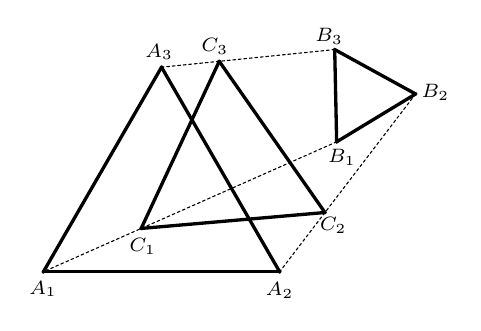
\begin{tikzpicture}[line cap=round,line join=round,>=triangle 45,x=1.0cm,y=1.0cm]
			\clip(-0.2,-0.4) rectangle (5.2,3.1);
			\draw [line width=1.2pt] (1.5,2.5980762113533165)-- (0.,0.);
			\draw [line width=1.2pt] (3.,0.)-- (1.5,2.5980762113533165);
			\draw [line width=1.2pt] (3.,0.)-- (0.,0.);
			\draw [line width=1.2pt] (3.699145393567602,2.822066217274539)-- (3.7242174909096546,1.6502204036531278);
			\draw [line width=1.2pt] (3.7242174909096546,1.6502204036531278)-- (4.726529686153215,2.257856383688207);
			\draw [line width=1.2pt] (4.726529686153215,2.257856383688207)-- (3.699145393567602,2.822066217274539);
			\draw [line width=0.4pt,dash pattern=on 1pt off 1pt] (3.699145393567602,2.822066217274539)-- (1.5,2.5980762113533165);
			\draw [line width=0.4pt,dash pattern=on 1pt off 1pt] (3.7242174909096546,1.6502204036531278)-- (0.,0.);
			\draw [line width=0.4pt,dash pattern=on 1pt off 1pt] (4.726529686153215,2.257856383688207)-- (3.,0.);
			\draw [line width=1.2pt] (2.2330484645225344,2.6727395466603907)-- (1.241405830303218,0.5500734678843759);
			\draw [line width=1.2pt] (1.241405830303218,0.5500734678843759)-- (3.575509895384405,0.7526187945627356);
			\draw [line width=1.2pt] (3.575509895384405,0.7526187945627356)-- (2.2330484645225344,2.6727395466603907);
			\begin{scriptsize}
				\draw [fill=black] (0.,0.) circle (0.5pt);
				\draw[color=black] (-0.005261746070665537,-0.21770732425839564) node {$A_1$};
				\draw [fill=black] (3.,0.) circle (0.5pt);
				\draw[color=black] (3.000102572819918,-0.2342810245463952) node {$A_2$};
				\draw [fill=black] (1.5,2.5980762113533165) circle (0.5pt);
				\draw[color=black] (1.4697975795612939,2.7937393596668647) node {$A_3$};
				\draw [fill=black] (3.7242174909096546,1.6502204036531278) circle (0.5pt);
				\draw[color=black] (3.79011561988123,1.4507118380668958) node {$B_1$};
				\draw [fill=black] (4.726529686153215,2.257856383688207) circle (0.5pt);
				\draw[color=black] (4.978455272126533,2.274430083976211) node {$B_2$};
				\draw [fill=black] (3.699145393567602,2.822066217274539) circle (0.5pt);
				\draw[color=black] (3.629903183763901,2.99262376312286) node {$B_3$};
				\draw [fill=black] (2.2330484645225344,2.6727395466603907) circle (0.5pt);
				\draw[color=black] (2.1769421251826078,2.8600341608188633) node {$C_3$};
				\draw [fill=black] (1.241405830303218,0.5500734678843759) circle (0.5pt);
				\draw[color=black] (1.2598640425799663,0.32370021848292416) node {$C_1$};
				\draw [fill=black] (3.575509895384405,0.7526187945627356) circle (0.5pt);
				\draw[color=black] (3.6796242846279,0.5888794230909175) node {$C_2$};
			\end{scriptsize}
		\end{tikzpicture}
	\end{figure}
	\item 设$\triangle A_1A_2A_3$, $\triangle B_1B_2B_3$与$\triangle C_1C_2C_3$均为正三角形($A_1$, $A_2$, $A_3$; $B_1$, $B_2$, $B_3$; $C_1$, $C_2$, $C_3$均按逆时针排列), $G_i$为$\triangle A_iB_iC_i$的重心($i=1, 2, 3$). 求证: $\triangle G_1G_2G_3$为正三角形. 
	\begin{figure}[H]
		\flushright
		\definecolor{uuuuuu}{rgb}{0.26666666666666666,0.26666666666666666,0.26666666666666666}
		\begin{tikzpicture}[line cap=round,line join=round,>=triangle 45,x=1.0cm,y=1.0cm]
			\clip(-0.3,-0.4) rectangle (5.6,4.7);
			\draw [line width=1.2pt] (1.5,2.5980762113533165)-- (0.,0.);
			\draw [line width=1.2pt] (3.,0.)-- (1.5,2.5980762113533165);
			\draw [line width=1.2pt] (3.,0.)-- (0.,0.);
			\draw [line width=1.2pt] (4.251265505253961,2.063337975764128)-- (4.092571439786291,0.9012487199079018);
			\draw [line width=1.2pt] (4.092571439786291,0.9012487199079018)-- (5.178317289556572,1.3448602557111817);
			\draw [line width=1.2pt] (5.178317289556572,1.3448602557111817)-- (4.251265505253961,2.063337975764128);
			\draw [line width=1.2pt] (2.59622559042284,2.7044938510189804)-- (4.154498551459449,3.023629466333357);
			\draw [line width=1.2pt] (4.154498551459449,3.023629466333357)-- (3.0989825208265165,4.213565628964271);
			\draw [line width=1.2pt] (3.0989825208265165,4.213565628964271)-- (2.59622559042284,2.7044938510189804);
			\draw [line width=0.4pt,dash pattern=on 1pt off 1pt] (1.5,2.5980762113533165)-- (4.251265505253961,2.063337975764128);
			\draw [line width=0.4pt,dash pattern=on 1pt off 1pt] (4.251265505253961,2.063337975764128)-- (3.0989825208265165,4.213565628964271);
			\draw [line width=0.4pt,dash pattern=on 1pt off 1pt] (3.0989825208265165,4.213565628964271)-- (1.5,2.5980762113533165);
			\draw [line width=0.4pt,dash pattern=on 1pt off 1pt] (4.092571439786291,0.9012487199079018)-- (0.,0.);
			\draw [line width=0.4pt,dash pattern=on 1pt off 1pt] (4.092571439786291,0.9012487199079018)-- (2.59622559042284,2.7044938510189804);
			\draw [line width=0.4pt,dash pattern=on 1pt off 1pt] (2.59622559042284,2.7044938510189804)-- (0.,0.);
			\draw [line width=0.4pt,dash pattern=on 1pt off 1pt] (4.154498551459449,3.023629466333357)-- (3.,0.);
			\draw [line width=0.4pt,dash pattern=on 1pt off 1pt] (4.154498551459449,3.023629466333357)-- (5.178317289556572,1.3448602557111817);
			\draw [line width=0.4pt,dash pattern=on 1pt off 1pt] (5.178317289556572,1.3448602557111817)-- (3.,0.);
			\draw [line width=1.2pt] (2.9500826753601594,2.9583266053605706)-- (2.2295990100697107,1.201914190308961);
			\draw [line width=1.2pt] (2.2295990100697107,1.201914190308961)-- (4.110938613672008,1.4561632406815135);
			\draw [line width=1.2pt] (4.110938613672008,1.4561632406815135)-- (2.9500826753601594,2.9583266053605706);
			\begin{scriptsize}
				\draw [fill=black] (0.,0.) circle (0.5pt);
				\draw[color=black] (-0.0024517495608417095,-0.1320761449051222) node {$A_1$};
				\draw [fill=black] (3.,0.) circle (0.5pt);
				\draw[color=black] (3.003832564254309,-0.15138846383755367) node {$A_2$};
				\draw [fill=black] (1.5,2.5980762113533165) circle (0.5pt);
				\draw[color=black] (1.3172233774886355,2.8098337724686058) node {$A_3$};
				\draw [fill=black] (4.092571439786291,0.9012487199079018) circle (0.5pt);
				\draw[color=black] (3.9758859505200217,0.7627279656308694) node {$B_1$};
				\draw [fill=black] (5.178317289556572,1.3448602557111817) circle (0.5pt);
				\draw[color=black] (5.353498034366793,1.3614098525362452) node {$B_2$};
				\draw [fill=black] (4.251265505253961,2.063337975764128) circle (0.5pt);
				\draw[color=black] (4.349257449880361,2.2304642044956613) node {$B_3$};
				\draw [fill=black] (2.59622559042284,2.7044938510189804) circle (0.5pt);
				\draw[color=black] (2.3794009187723613,2.8484584103334685) node {$C_1$};
				\draw [fill=black] (4.154498551459449,3.023629466333357) circle (0.5pt);
				\draw[color=black] (4.2913204930830675,3.1574555132523723) node {$C_2$};
				\draw [fill=black] (3.0989825208265165,4.213565628964271) circle (0.5pt);
				\draw[color=black] (3.0810818399840345,4.464255761013568) node {$C_3$};
				\draw [fill=uuuuuu] (2.9500826753601594,2.9583266053605706) circle (0.5pt);
				\draw[color=uuuuuu] (2.978082805677734,3.196080151117235) node {$G_3$};
				\draw [fill=uuuuuu] (2.2295990100697107,1.201914190308961) circle (0.5pt);
				\draw[color=uuuuuu] (2.0575289365651717,1.1554117839236429) node {$G_1$};
				\draw [fill=uuuuuu] (4.110938613672008,1.4561632406815135) circle (0.5pt);
				\draw[color=uuuuuu] (4.011291868562813,1.293816736272735) node {$G$};
			\end{scriptsize}
		\end{tikzpicture}
	\end{figure}
\end{enumerate}
\end{document}